% chap3.tex (Definitions and Theorem)

\chapter{Sensor Data Provenance Collection Framework for the IoT}

In this chapter, we define how provenance is collected and modeled along the IoT architectural stack. We also define implementation specifics of the provenance collection framework for IoT device. 

\section{IoT Provenance-Collection framework Information flow}
%This section discusses the data model in which we represent sensor and actuator reading of provenance data collected from IoT devices . It also talks about the relationship between IoT provenance Collection and PROV\-DM; How data is process and dissemenated accross the IoT architecture.
%
%\textcolor{red}{TODO: Talks about how we use PROV\-DM and what kinds of provenance we are looking to store}

A provenance model is used to represent causal relationship between objects and it is usually modeled as a Directed Acyclic Graph(DAG). This enables for better graphical representation of provenance relationships and also a unified format for representing provenance data. There are two major models for representing provenance, OPM and Prov-DM. PROV-DM is a predecessor and standardized version of OPM. It allows the modeling of data objects either physical or digital. PROV-DM is chosen as the model to represent provenance for our implementation because it allows for proper representation of all of the relationships in which we envision for IoT devices. This section defines a model for relaying provenance in IoT systems which is built on top of PROV-DM. 
From the IoT architecture as described in Section 2, we can see that data is disseminated from sensors and actuators across various layers contained in the IoT architectural stack. The provenance data produced from various sensors is collectively aggregated at the gateway layer and/or the cloud layer. We allow for provenance data to be translated to the appropriate PROV\-DM format at the various levels of the IoT architecture. This allows for fault tolerant processing of information even in the case of a network failure at all layers. Sensor readings are collected from devices as specified by a policy. This helps address the issue with memory constraint  of collecting provenance data in IoT devices. Policy specification and implementation  are discussed in greater detail in chapter 4.  Figure 4.1 illustrates the data aggregation at various layers of the IoT architectural stack.


\begin{figure}[h!]
\begin{center}

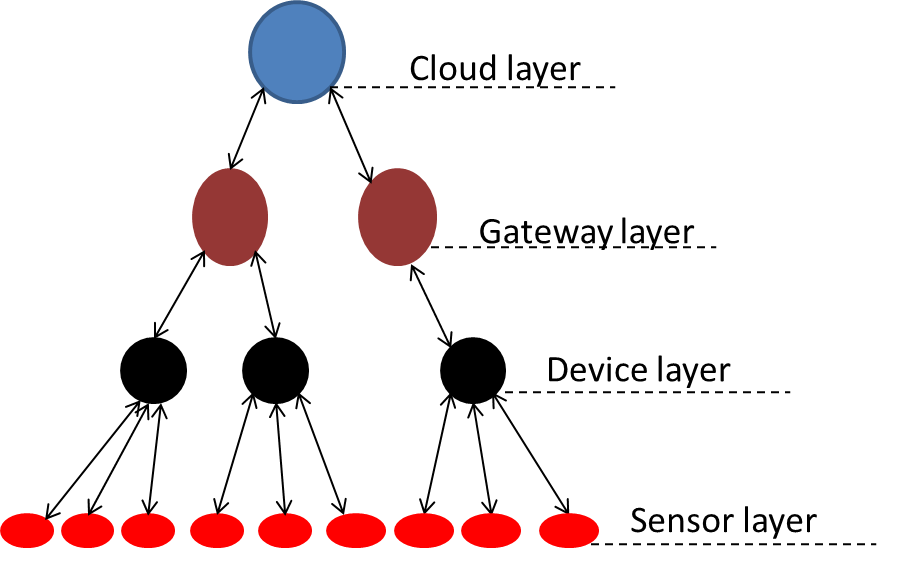
\includegraphics[width=3.0in]{iot.PNG}    
\end{center}
\caption{IoT provenance-collection data aggregation}
\label{autom}
\end{figure}


Using the scenario of a smart home use case as described in chapter 2, a detailed example of how our provenance collection framework can be applied is described below

\begin{itemize}

\item Provenance data is collected from sensors and actuator readings of devices contained in the smart home(e.g thermostat, refrigerator, and smart doors). The provenance data is collected as specified in a policy document. Policy document contains information of which provenance data to be collected in the device and can be only be defined by the device owner(e.g house owner). 

\item Provenance data from each device is aggregated and passed along to the gateway. The information is further analyzed and transmitted to the cloud for storage in which further analysis could be conducted on the data to derive more insights from the provenance data collected. The gateway collectively aggregates data from multiple sensors and forwards the aggregated data to the cloud for further processing. This information is then transferred to the cloud where it is mapped using the PROV\-DM which allows for causal relationship between the objects contained in the IoT framework. The cloud contains all of the aggregated provenance data from the respective devices contained in the smart home in which further analysis can be performed on the collective provenance data. 


Each layer in the provenance IoT architecture is indepent of the and maintains provenance information that can be mapped using the PROV\-DM format which allows for the representation of dependencies that exists between objects contained in the device. This allows for provenance data to be further analyzed at the respective layers even in an event of network loss. 



\end{itemize}





\subsection{Provenance-Collection Model Definition}

It is assumed that provenance data is collected from the underlying IoT device using the framework outline in section 3 of this chapter below. Data is collected from sensors and actuators attached to an IoT device. The underlying construct is represented as a acyclic graph which denotes the relationship between multiple sensors and actuator readings. Since PROV-DM type provides a generic model for relaying provenance information, we define a more specific construct for representing provenance data in IoT devices based on  PROV-DM. In the context of IoT provenance entity, process and agent are defined as follows:

\begin{itemize}

\item Agent: An agent contains information on an object that accesses an entity. Examples of agents in an IoT architecture are sensors, actuators, user roles(e.g admin). A unique identifier is given to each agents contained in the IoT framework.

\item Entity:  An entity can be defined as a data object that contains information which can be modified. An example entities are device files, processes, device memory contents.

\item Activity: An activity is a modification that an agent makes on an entity. An example of an activity are basic file access modifications such as read, write, delete, update. 


\end{itemize}


To better emphasize the provenance-collection model, an example of a use case for the provenance collection model is illustrated in the figure below.



\begin{figure}[h]
\begin{center}

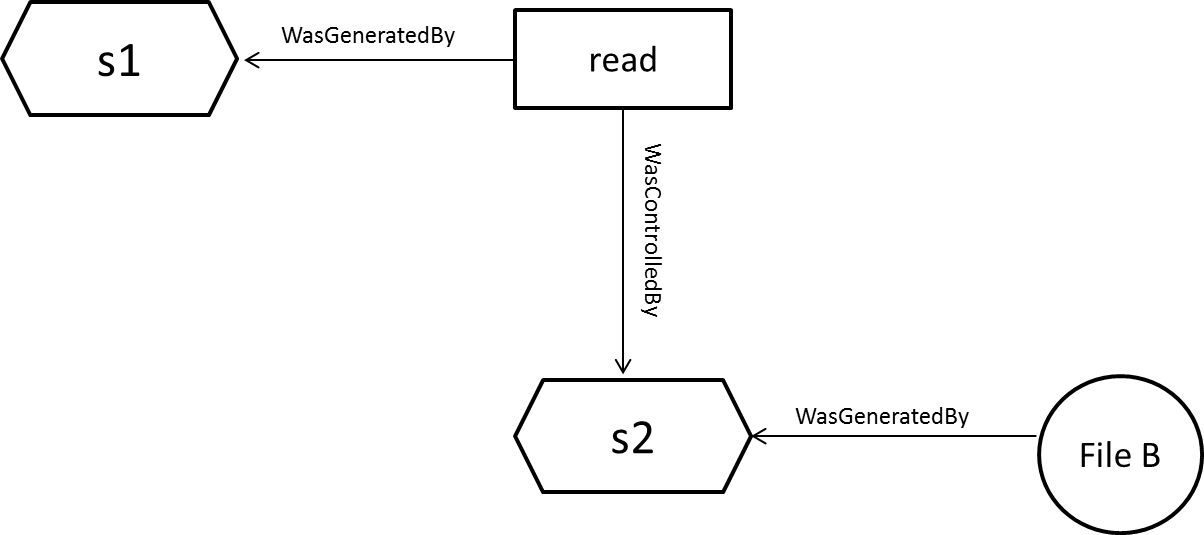
\includegraphics[width=3.0in]{usecase.png}    
\end{center}
\caption{Provenance-model use case}
\label{autom}
\end{figure}





The figure above depicts a dependency relationship between two sensors, s1 and s2. Consider the scenario of a smart home in which, s1 is smart thermostat contained in a smart home which regulates the temperature of the home and s2 is a sensor that detects the temperature outside of the house. s1 constantly checks the temperature outside to regulate the temperature of the house accordingly. s1 tries to access information from s2. According to the provenance data model  definition, s1 and s2 are agents. The activity performed on s2 by s1 is read. File B is the entity in which s1 tries to read from s2 to determine the environment temperature. The relationship between various components contained in the model is illustrated on the edges of the graph.

\par The relations which defines the relationship between types of a provenance model. We use the same instance of the relations contained in prov-dm to represent relationships between types contained in the IoT framework.


\section{Provenance-Collection System}

In this section, we outline the components of our system and describe how provenance trace is collected across the IoT framework. Figure 1 displays the system architecture of our approach. Sensor and actuator readings in the form of Input and output(I/O) trace are recorded by the tracer component. This component intercepts system level I/O events and produces trace information in the Common Trace Format (CTF). CTF represents binary trace output information containing multiple streams of binary events such as I/O activity. Trace information is converted into the PROV-DM and serialized to PROV-JSON. This represents the relationship between provenance entities contained in the system. CTF conversion to OPM will be achieved using babeltrace. Babeltrace is a plugin which allows the ocnversion of CTF trace into various readable format. It includes plugins in which CTF trace data can be intercepted to create a custom conversion format. Our system relies heavily on data pruning to reduce and remove unimportant provenance in order to conserve memory and address the memory constraint issues faced by low memory embedded systems. This is achieved by using a policy-based approach in which a user with administrative privilege is given permission to create or modify a policy. This policy document dictates what provenance data to collect. Pruned provenance from the device is securely transmitted to a gateway and later transmitted and stored in a private cloud backend. The backend of choice is Neo4j, a graph database for efficient storage, query and visualization of provenance graph data.

\begin{figure}[h]
\begin{center}

\includegraphics[width =3.0in]{architecture.PNG}    
\end{center}
\caption{Proposed Model}
\label{autom}
\end{figure}

The goal is to create a provenance\-aware system which records I/O operations on data for devices connected in an IoT system. For our implementation, several tools and hardware components are utilized in the development of our prototype, some of the tools utilized are outlined below:

\begin{itemize}
\item BeagleBone Black Board. This device is a microcontroller used to evaluate our approach. We choose the BeagleBone Board because it is a representation of what can be found on an IoT gateway device and it has the capability to include custom hardware in programmable logic. Also, BeagleBone is a low­cost, simple IoT demonstrator that was chosen for its high­ performance, on­board emulation, and IoT gateway projects can be programmed without additional need for hardware tools.

%\item Real Time Executive for Multiprocessor Systems (RTEMS) is an open source real­time operating system (RTOS) for embedded systems. This operating system is a typical RTOS that may be deployed in IoT devices.

\item Neo4j, a graph database which allow the optimized querying of graph data. Since provenance represents causal dependencies, it is ideal to use a graph database to store the relationships between objects

\item lttng, a software tool for collecting system level trace on Linux system. 

\end{itemize}


\section{Experiment Evaluation}

I plan to evaluate the effectiveness of our approach for the provenance collection framework by implementing an intrusion detection system for IoT device. An IDS is used to detect malicious attacks based on a certain policy or threshold set by an administrator. There are two types of  IDS: Rule-based approach, or anomaly based approach. The rule based approach allows for intrusion monitoring based on rules specified by an administrator. On the other hand, anomaly based IDS which monitors intrusion based on patterns that falls out of the normal system function. Most anomaly\-based approach deals with machine learning to classify normal or anomalous behavior. Provenance collection IDS system uses provenance data to provide intrusion detection capabilities in the IoT framework. It follows a rule based approach in which when provenance  I plan to test the throughput and precision recall on the detection rate. We will evaluate ur provenance collection system using the work of Xie et al. Xie et al proposes an intrusion detection system which uses system level provenance data to provide vulnerability intrusion detection. The system collects provenance, detects intrusion and analyzes vulnerabilities that exists based on provenance data.  


%\section{Provenance Aware IDS System for IoT }
%
%This section outlines the core functionalities of our model PAIST. 
